\documentclass[12pt]{article}
\usepackage{geometry}                % See geometry.pdf to learn the layout options. There are lots.
\geometry{letterpaper}                   % ... or a4paper or a5paper or ... 
%\geometry{landscape}                % Activate for for rotated page geometry
\usepackage[parfill]{parskip}    % Activate to begin paragraphs with an empty line rather than an indent
\usepackage{daves,fancyhdr,natbib,graphicx,dcolumn,amsmath,lastpage,url}
\usepackage{amsmath,amssymb,epstopdf,longtable}
\usepackage{paralist}  % need to modify standard enumerate blocks
\usepackage[final]{pdfpages}
\DeclareGraphicsRule{.tif}{png}{.png}{`convert #1 `dirname #1`/`basename #1 .tif`.png}
\pagestyle{fancy}
\lhead{CE 3354 -- Engineering Hydrology}
\rhead{SUMMER 2025}
\lfoot{ES3}
\cfoot{}
\rfoot{Page \thepage\ of \pageref{LastPage}}
\renewcommand\headrulewidth{0pt}



\begin{document}
\begin{center}
{\textbf{{ CE 3354 Engineering Hydrology} \\ {Exercise Set 3}}}
\end{center}

 \section*{\small{Exercises}}
 \begin{enumerate}

\item Estimate the monthly evapotranspiration depths for Dallas (Tarrant County), Houston (Harris County), and San Angelo (Concho County) area using the Blaney-Criddle method.\footnote{A Google search should get you sufficient guidance to perform this exercise.}

Solution(s):

We will need some city specific geographic data

\begin{figure}[h!] %  figure placement: here, top, bottom, or page
   \centering
   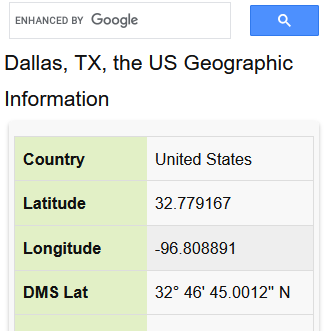
\includegraphics[height=2in]{dallaslatitude.png} 
   \caption{Latitude for Dallas, Texas}
   \label{fig:dallas-lat}
\end{figure}
\begin{figure}[h!] %  figure placement: here, top, bottom, or page
   \centering
   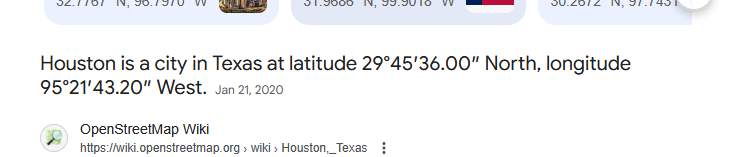
\includegraphics[width=4in]{houstonlatitude.png} 
   \caption{Latitude for Houston, Texas}
   \label{fig:houston-lat}
\end{figure}
\begin{figure}[h!] %  figure placement: here, top, bottom, or page
   \centering
   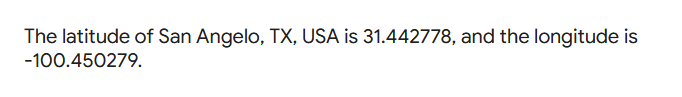
\includegraphics[width=4in]{sanangelolat.png} 
   \caption{Latitude for San Angelo, Texas}
   \label{fig:sanangelo-lat}
\end{figure}

Then some temperature data

\begin{figure}[h!] %  figure placement: here, top, bottom, or page
   \centering
   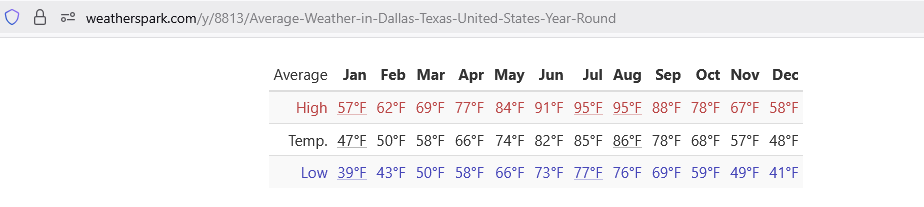
\includegraphics[width=6in]{mmtdallas.png} 
   \caption{Mean Monthly Air Temperature for Dallas, Texas}
   \label{fig:mmtdallas}
\end{figure}

\begin{figure}[h!] %  figure placement: here, top, bottom, or page
   \centering
   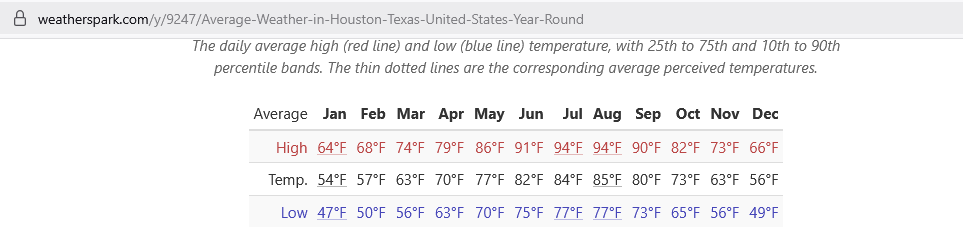
\includegraphics[width=6in]{houstonmmt.png} 
   \caption{Mean Monthly Air Temperature for Houston, Texas}
   \label{fig:mmthouston}
\end{figure}

\begin{figure}[h!] %  figure placement: here, top, bottom, or page
   \centering
   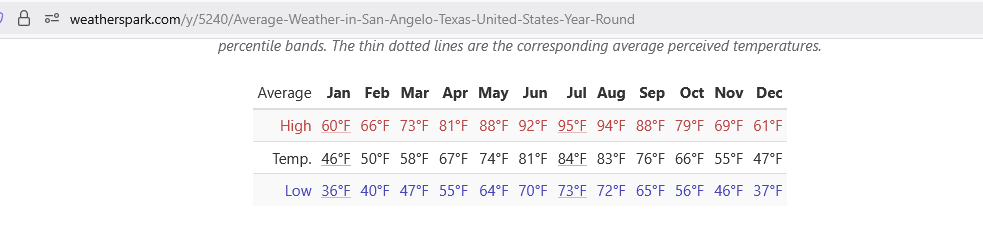
\includegraphics[width=6in]{mmtsanangelo.png} 
   \caption{Mean Monthly Air Temperature for San Angelo, Texas}
   \label{fig:mmtsanangelo}
\end{figure}

Now have data to employ the spreadsheet implementation; we should probably note units on the spreadsheet - based on class notes the values $ET_o$ are in millimeters per day, so monthly depths would be these values multiplied 30 (for typical month length)

\begin{figure}[h!] %  figure placement: here, top, bottom, or page
   \centering
   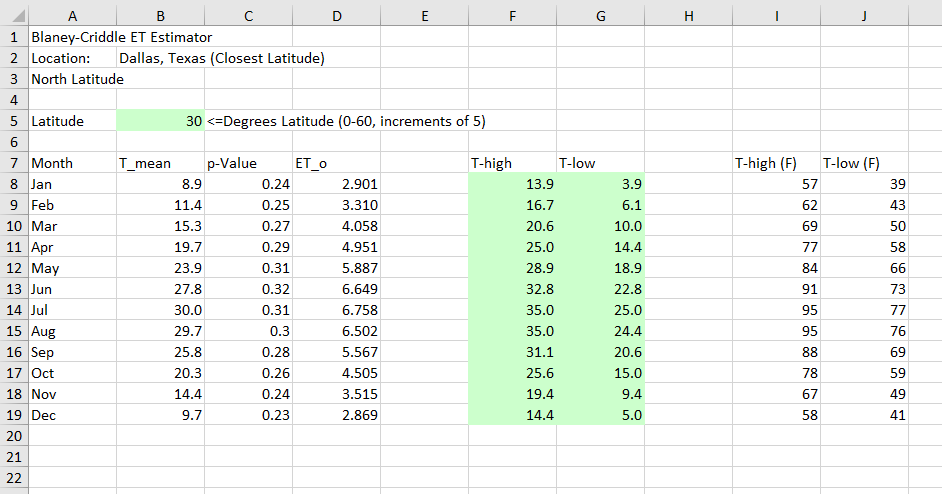
\includegraphics[width=6in]{bcdallas.png} 
   \caption{Blaney-Criddle evapotranspiration for Dallas, Texas}
   \label{fig:bcdallas}
\end{figure}

\begin{figure}[h!] %  figure placement: here, top, bottom, or page
   \centering
   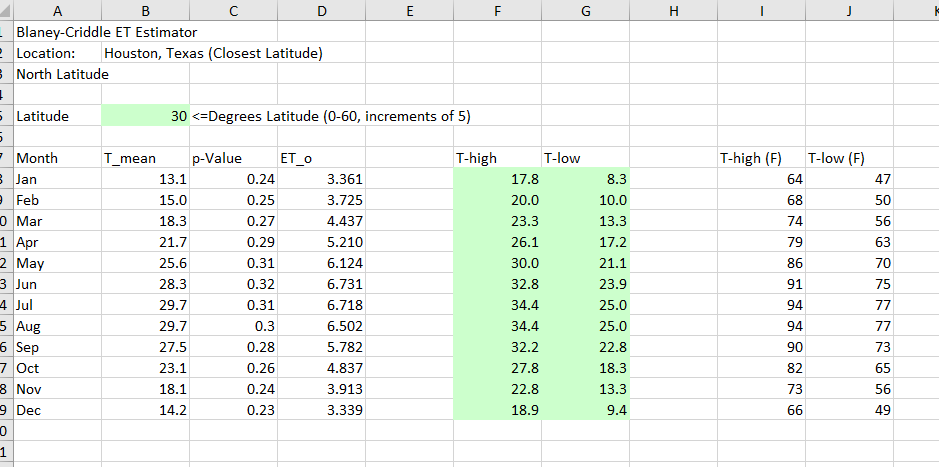
\includegraphics[width=6in]{bchouston.png} 
   \caption{Blaney-Criddle evapotranspiration for Houston, Texas}
   \label{fig:bchouston}
\end{figure}

\begin{figure}[h!] %  figure placement: here, top, bottom, or page
   \centering
   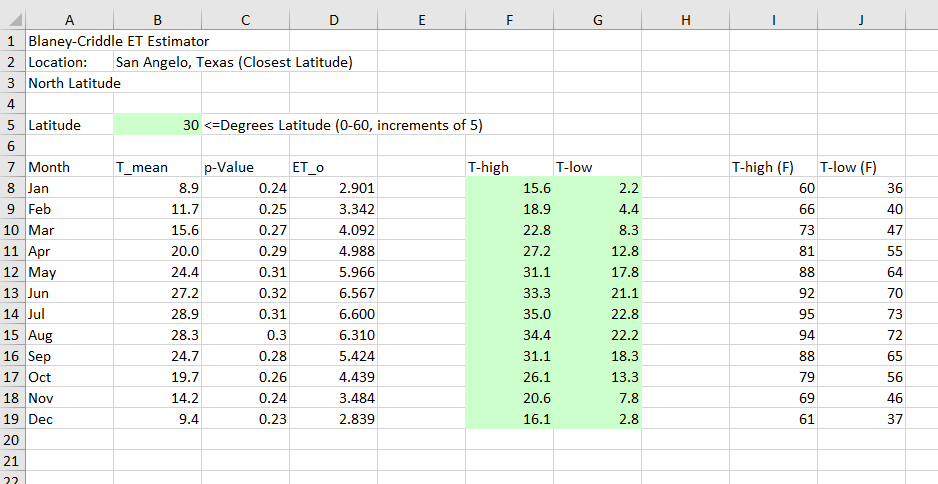
\includegraphics[width=6in]{bcsanangelo.png} 
   \caption{Blaney-Criddle evapotranspiration for San Angelo, Texas}
   \label{fig:bcsanangelo}
\end{figure}

\clearpage
%%%%%%%%%%%%%%%%%%%%%%%%%%%%%%%%%%%%%%%%%%%%%%%%%%%%%%%%%%%%%%%%%%%%%%%%%%%%%%%%%%%%%%%%%%
\item Estimate the monthly evapotranspiration depths for the San Angelo (Concho County) area using the Thornwaithe method.\footnote{A Google search should get you sufficient guidance to perform this exercise.}

Solution(s):

Using same data sources, but a different tool we obtain

\begin{figure}[h!] %  figure placement: here, top, bottom, or page
   \centering
   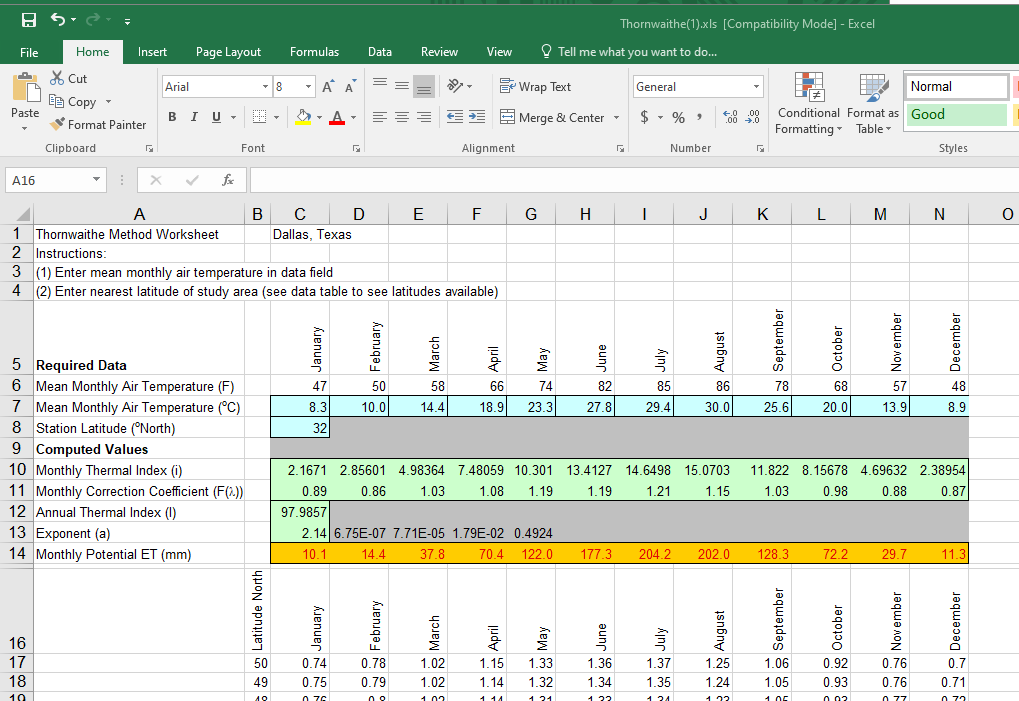
\includegraphics[width=6in]{thorndallas.png} 
   \caption{Thornwaithe evapotranspiration for Dallas, Texas}
   \label{fig:thorndallas}
\end{figure}

\begin{figure}[h!] %  figure placement: here, top, bottom, or page
   \centering
   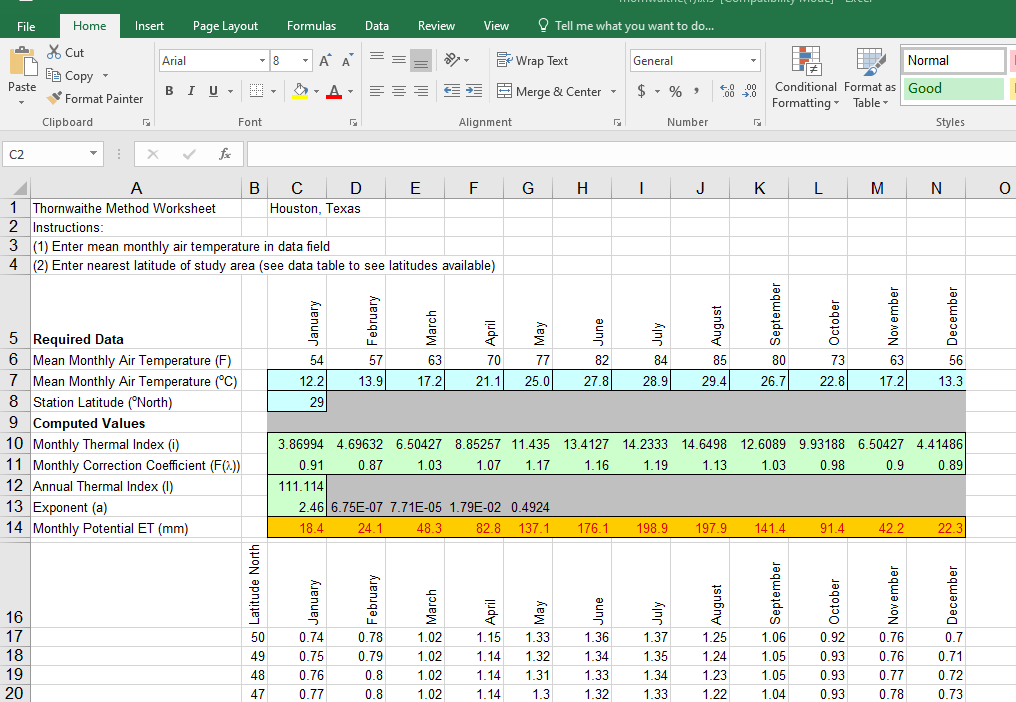
\includegraphics[width=6in]{thornhouston.png} 
   \caption{Thornwaithe evapotranspiration for Houston, Texas}
   \label{fig:thornhouston}
\end{figure}

\begin{figure}[h!] %  figure placement: here, top, bottom, or page
   \centering
   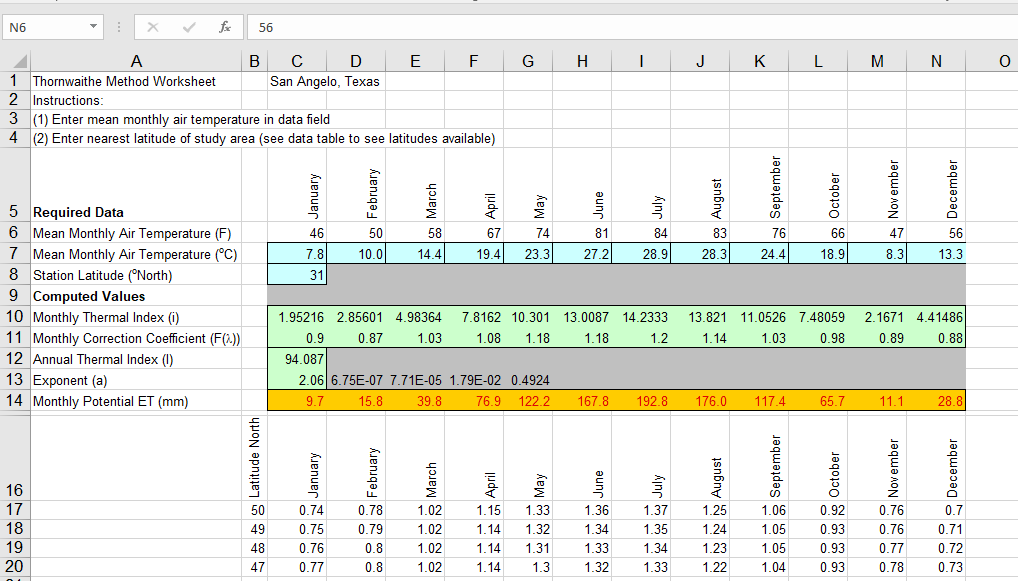
\includegraphics[width=6in]{thornsanangelo.png} 
   \caption{Thornwaithe evapotranspiration for San Angelo, Texas}
   \label{fig:thornsanangelo}
\end{figure}

\clearpage
%%%%%%%%%%%%%%%%%%%%%%%%%%%%%%%%%%%%%%%%%%%%%%%%%%%%%%%%%%%%%%%%%%%%%%%%%%%%%%%%%%%%%%%%%%
\item Locate grid cells 506,410, and 812 at the TWDB lake evaporation database. Determine the long term monthly evaporation rates for the three cells.  Compare these rates to the estimates you made above.  These cells correspond approximately to

\begin{itemize}
\item 410 == Dallas
\item 812 == Houston
\item 506 == San Angelo
\end{itemize}

Solution(s):

The next several pages show how to accomplish the database manipulation using ENGR-1330 methods.

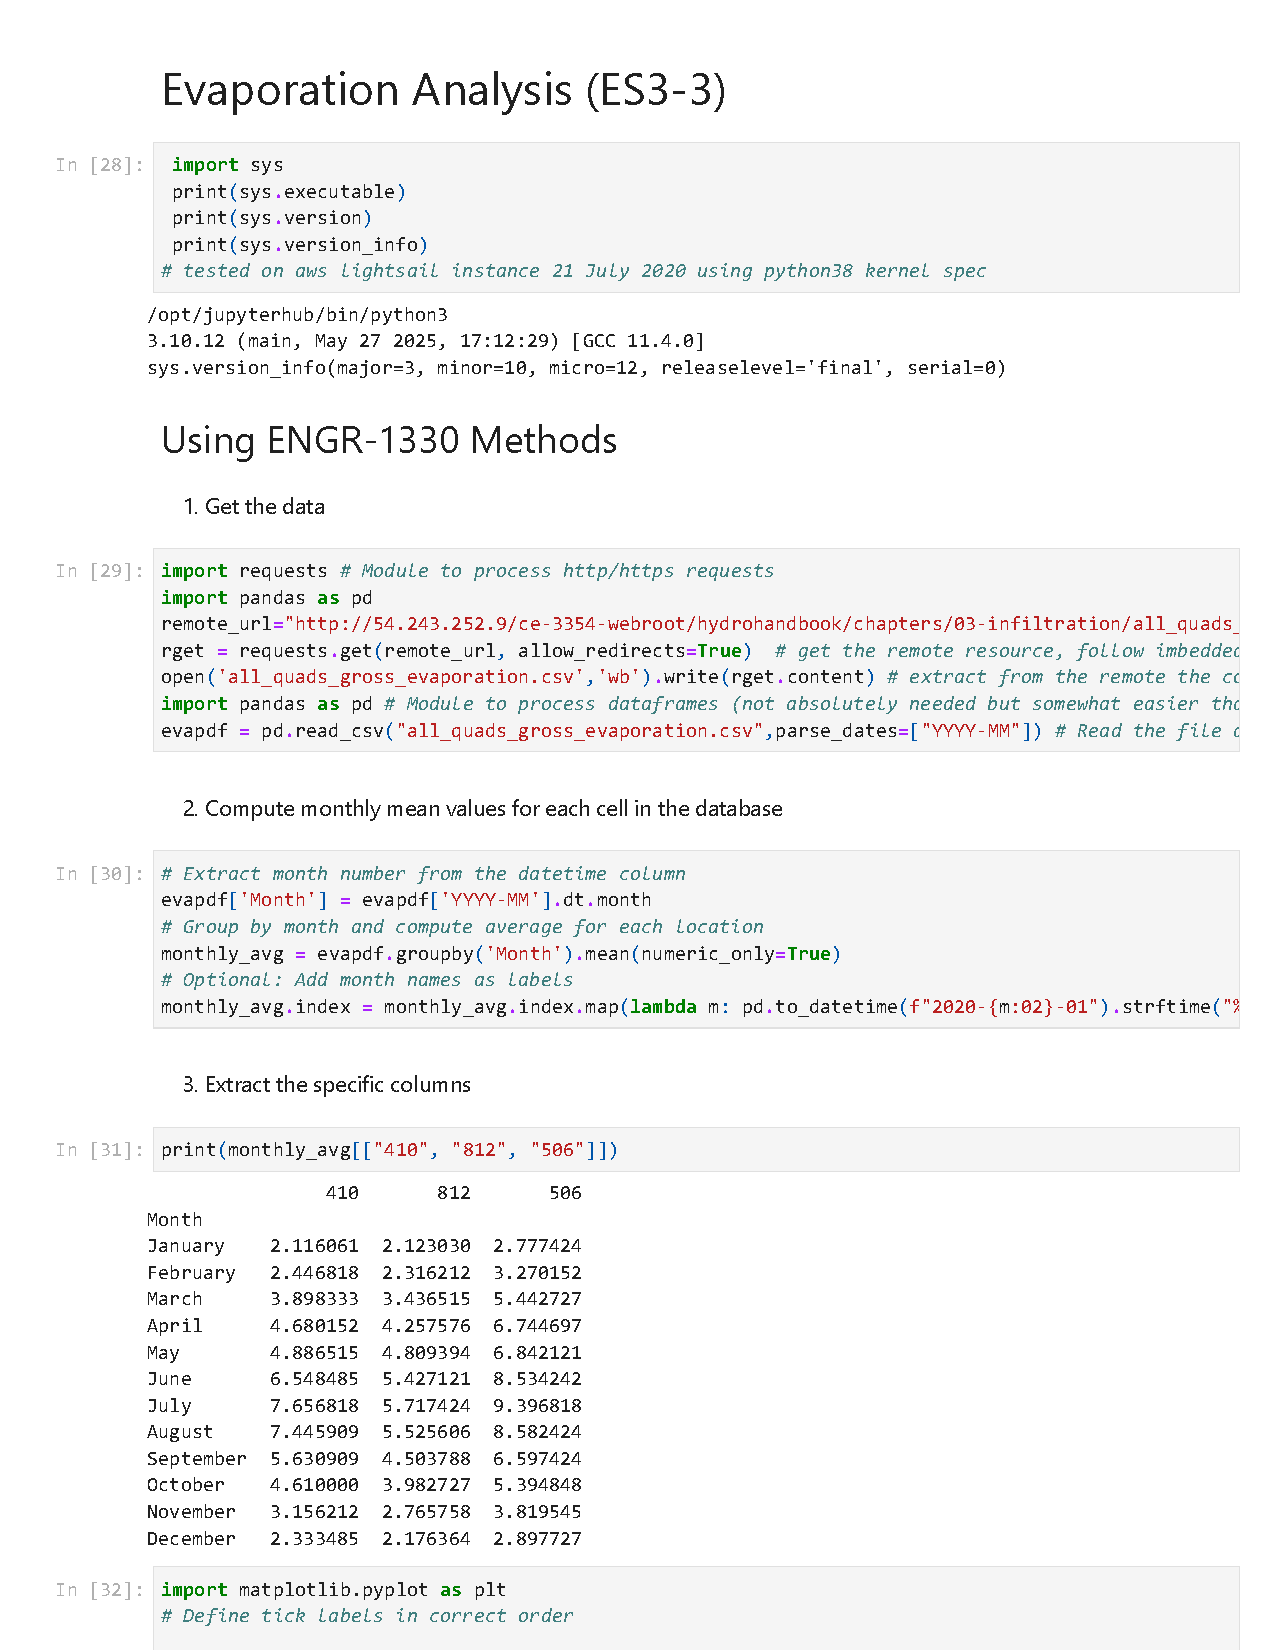
\includepdf[pages={-}]{./EvaporationAnalysisHomework.pdf}

Comparing all the methods (for a summer month); The data science approach for July is 7-9 inches for the month, Thornwaithe is 192-204 millimeters, about 7.5-8.03 inches so comparable, Blaney-Criddle is 198-202 millimeters, about 7.8-7.9 inches, also comparable.

All methods return about same values for the region (at least for July) - the data science results have the advantage of being derived from actual measured values.

\clearpage
%%%%%%%%%%%%%%%%%%%%%%%%%%%%%%%%%%%%%%%%%%%%%%%%%%%%%%%%%%%%%%%%%%%%%%%%%%%%%%%%%%%%%%%%%
\item A storm of moderate intensity strikes a semi-urban watershed with predominantly loamy soils. The storm begins at time $ t = 0 $ and lasts for \textbf{3 hours} with a constant rainfall intensity of \textbf{15 mm/h}.

The watershed has the following properties:

\begin{itemize}
    \item Area: 2 hectares
    \item Slope: gentle (assume negligible effect)
    \item Vegetative cover: 50\% grass, 50\% compacted dirt
    \item Antecedent moisture conditions: dry (unless otherwise specified)
    \item Initial abstraction: assume 5 mm where applicable
\end{itemize}

A prior study suggests the following Horton parameters:
\begin{align*}
    f_0 &= 5\ \text{mm/h} \quad \text{(initial infiltration capacity)} \\
    f_c &= 1\ \text{mm/h} \quad \text{(final infiltration capacity)} \\
    k   &= 2.0\ \text{h}^{-1} \quad \text{(decay constant)}
\end{align*}


Determine:
\begin{enumerate}[a)]
    \item The infiltration rate function $f(t)$ over the 3-hour duration using Horton’s exponential decay equation: $f(t) = f_c + (f_0 - f_c) e^{-kt}$
    \item The cumulative infiltration depth $F(t)$, by integrating the rate function over time.
    \item Plot the rate and cumulative infiltration depth for every 15-minutes for the 3 hour storm.
    \item Report the total runoff depth as: $\text{Runoff} = \text{Rainfall Depth} - F(3\ \text{h})$
\end{enumerate}

Solution(s):

a) Substitute supplied values: 
$$f(t) = 1.0~\text{mm/hr} + (5.0~\text{mm/hr} - 1.0~\text{mm/hr}) \cdot e^{-2.0~\text{hr}^{-1}~t}$$

This function gets encoded into a spreadsheet.

b) We are given the function:

$$
f(t) = f_c + (f_o - f_c) e^{-k t}
$$

where:
\begin{itemize}
    \item \( f_c \) is a constant (final value),
    \item \( f_o \) is a constant (initial value),
    \item \( k \) is a time constant,
    \item \( t \) is time.
\end{itemize}

We wish to compute the indefinite integral (antiderivative) of \( f(t) \):

\[
F(t) = \int f(t)\, dt = \int \left[ f_c + (f_o - f_c) e^{-kt} \right] dt
\]

We break this into parts and integrate term by term:

\[
= f_c \int dt + (f_o - f_c) \int e^{-kt} dt
\]

Now integrate:

\[
= f_c t - \frac{f_o - f_c}{k} e^{-kt} + C
\]

where \( C \) is the constant of integration, its value determined from $F(0)=0$

%\bigskip
%\noindent\textbf{Final Result:}
\[
\boxed{ F(t) = \int f(t)\, dt = f_c t - \frac{f_o - f_c}{k} e^{-kt} + C }
\] 

This function also gets encoded into a spreadsheet.
\clearpage
c) and d) These two components are shown directly in the solution spreadsheet (Figures \ref{fig:es3-4xls} and \ref{fig:es3-4func})

\begin{figure}[h!] %  figure placement: here, top, bottom, or page
   \centering
   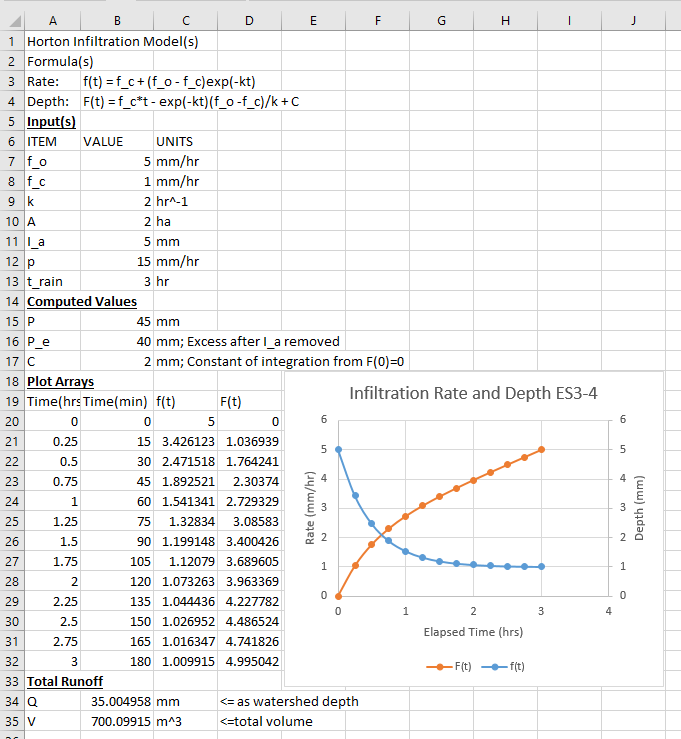
\includegraphics[width=6in]{es3-4xls.png} 
   \caption{Excel screen capture for ES3-4}
   \label{fig:es3-4xls}
\end{figure}
\clearpage
\begin{figure}[h!] %  figure placement: here, top, bottom, or page
   \centering
   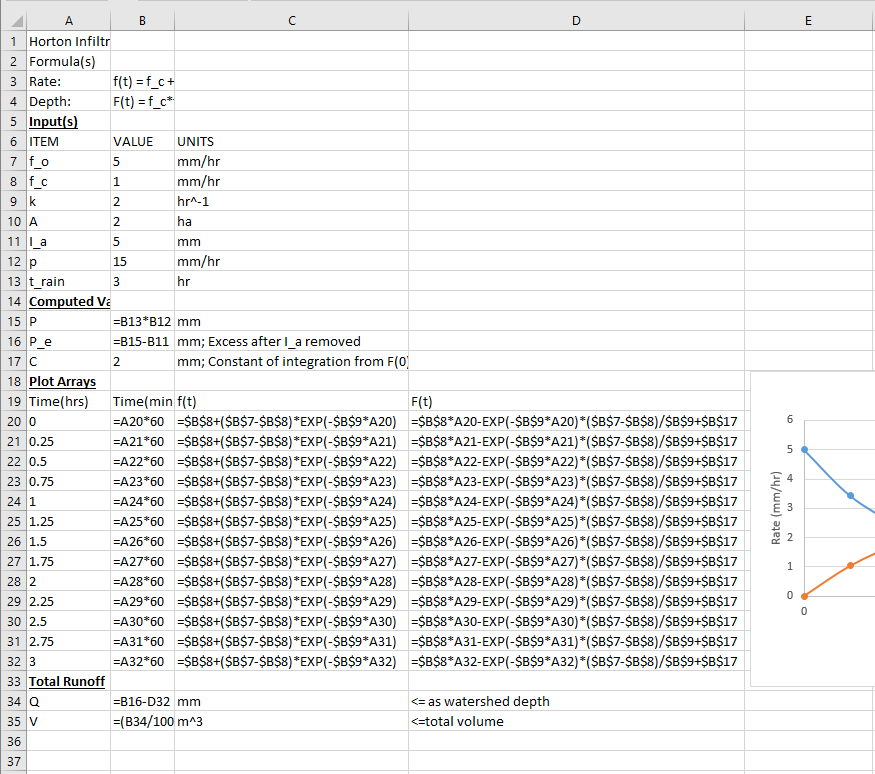
\includegraphics[width=6in]{es3-4func.png} 
   \caption{Excel screen capture for ES3-4 (formulas)}
   \label{fig:es3-4func}
\end{figure}

\clearpage
%%%%%%%%%%%%%%%%%%%%%%%%%%%%%%%%%%%%%%%%%%%%%%%%%%%%%%%%%%%%%%%%%%%%%%%%%%%%%%%%
\item A storm of moderate intensity strikes a semi-urban watershed with predominantly loamy soils. The storm begins at time $ t = 0 $ and lasts for \textbf{3 hours} with a constant rainfall intensity of \textbf{15 mm/h}.

The watershed has the following properties:

\begin{itemize}
    \item Area: 2 hectares
    \item Slope: gentle (assume negligible effect)
    \item Vegetative cover: 50\% grass, 50\% compacted dirt
    \item Antecedent moisture conditions: dry (unless otherwise specified)
    \item Initial abstraction: assume 5 mm where applicable
\end{itemize}

An prior study suggests the following Green-Ampt parameters for the watershed:
\begin{align*}
    \Delta \theta &= 0.25 \quad \text{(initial moisture deficit)} \\
    \psi &= 110\ \text{mm} \quad \text{(wetting front suction head)} \\
    K_s &= 3\ \text{mm/h} \quad \text{(saturated hydraulic conductivity)}
\end{align*}

Determine:
\begin{enumerate}[a)]
     \item Use the Green-Ampt equation to estimate cumulative infiltration: 
     $$F = K_s t + \psi \Delta \theta \ln \left(1 + \frac{F}{\psi \Delta \theta} \right)$$ 
     Solve this equation iteratively (numerically or in Excel/Python) for $ t = 3 $ hours.
    \item Plot the Green-Ampt cumulative infiltration for every 15-minutes for the 3 hour storm.
    \item Report the total runoff depth as: $\text{Runoff} = \text{Rainfall Depth} - F(3\ \text{h})$
\end{enumerate}

Solution(s):

a) We are given the following nonlinear equation that relates cumulative infiltration \( F \) to time \( t \):

\[
F = K_s t + \psi \Delta \theta \ln \left(1 + \frac{F}{\psi \Delta \theta} \right)
\]

\noindent where:
\begin{itemize}
    \item \( K_s \) is the saturated hydraulic conductivity \((\text{L/T})\),
    \item \( \psi \) is the capillary suction head \((\text{L})\),
    \item \( \Delta \theta \) is the change in moisture content (dimensionless),
    \item \( t \) is time \((\text{T})\),
    \item \( F \) is the cumulative infiltration \((\text{L})\).
\end{itemize}

\noindent This equation cannot be solved explicitly for \( F \) because it appears on both sides of the equation and inside a logarithm. However, we can solve it numerically using an iterative approach or a root-finding method.

\subsubsection*{Numerical Solution Strategy}

We recast the equation as a root-finding problem by defining a residual function:

\[
f(F_{\text{guess}}) = F_{\text{guess}} - \left[ K_s t + \psi \Delta \theta \ln \left(1 + \frac{F_{\text{guess}}}{\psi \Delta \theta} \right) \right]
\]

\noindent We then seek the value of \( F_{\text{guess}} \) such that \( f(F_{\text{guess}}) = 0 \).

\subsubsection*{Solving in Excel Using Goal Seek}

To solve the equation for a fixed time \( t = 3 \) hours using Excel:

\begin{enumerate}
    \item Create input cells for:
    \begin{itemize}
        \item \( K_s \)
        \item \( \psi \)
        \item \( \Delta \theta \)
        \item \( t = 3 \)
    \end{itemize}
    \item Create a cell labeled \texttt{F\_guess} and assign it an initial value (e.g., 5 cm).
    \item In another cell, compute the right-hand side of the equation:
    \[
    F(t) = K_s \cdot t + \psi \cdot \Delta \theta \cdot \ln\left(1 + \frac{\texttt{F\_guess}}{\psi \cdot \Delta \theta} \right)
    \]
    \item Compute the residual in a separate cell:
    \[
    \texttt{Residual} = \texttt{F\_guess} - F(t)
    \]
    \item Use Excel's \textbf{Goal Seek}:
    \begin{itemize}
        \item Set \texttt{Residual} to 0
        \item By changing \texttt{F\_guess}
    \end{itemize}
\end{enumerate}

\noindent This process will return the value of \( F \) that satisfies the infiltration equation for the given parameters.

b) and c) Figures \ref{fig:es3-5xls} and \ref{fig:es3-5func} are the spreadsheet that performs the calculations.  The Goal Seek portion is done row-by-row; the process could be automated by using the Excel Macro recorder.

\begin{figure}[h!] %  figure placement: here, top, bottom, or page
   \centering
   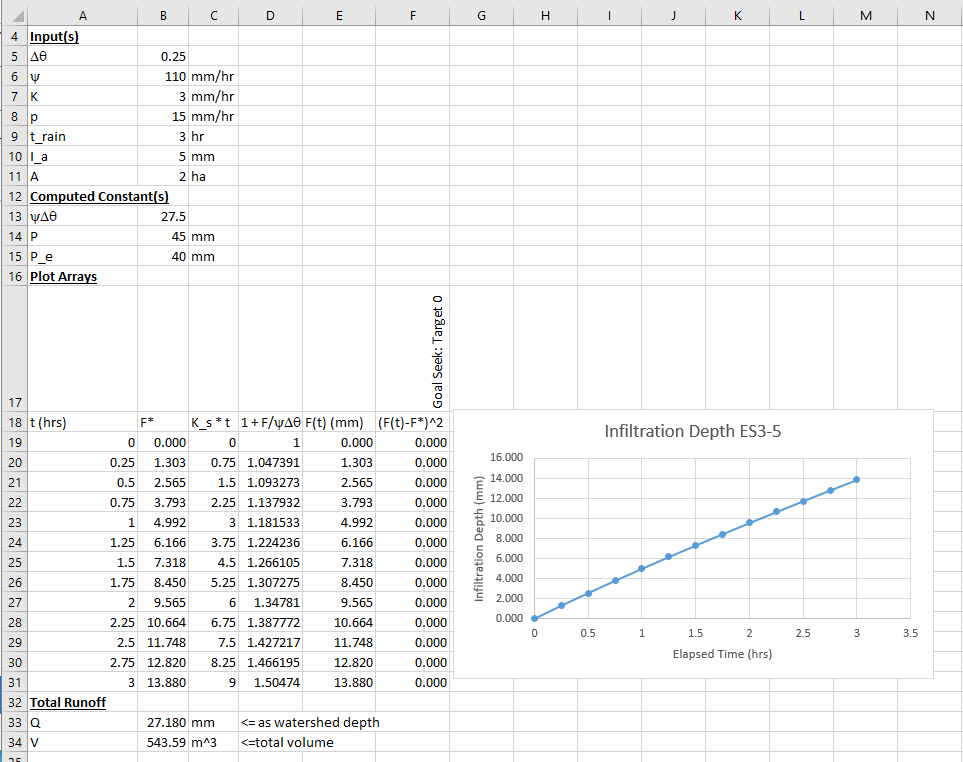
\includegraphics[width=6in]{es3-5xls.png} 
   \caption{Excel screen capture for ES3-5}
   \label{fig:es3-5xls}
\end{figure}
\clearpage
\begin{figure}[h!] %  figure placement: here, top, bottom, or page
   \centering
   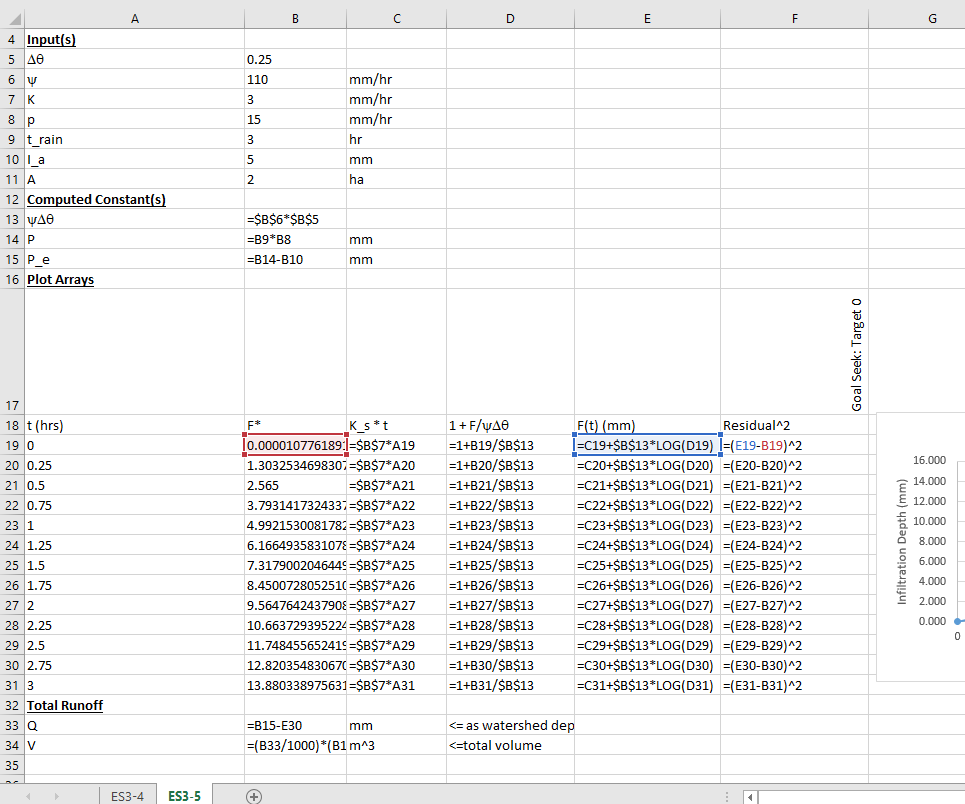
\includegraphics[width=6in]{es3-5func.png} 
   \caption{Excel screen capture for ES3-5 (formulas)}
   \label{fig:es3-5func}
\end{figure}
\clearpage
%%%%%%%%%%%%%%%%%%%%%%%%%%%%%%%%%%%%%%%%%%%%%%%%%%%%%%%%%%%%%%%%%%%%%%%%%%%%%%%
\item A storm of moderate intensity strikes a semi-urban watershed with predominantly loamy soils. The storm begins at time $ t = 0 $ and lasts for \textbf{3 hours} with a constant rainfall intensity of \textbf{15 mm/h}.

The watershed has the following properties:

\begin{itemize}
    \item Area: 2 hectares
    \item Slope: gentle (assume negligible effect)
    \item Vegetative cover: 50\% grass, 50\% compacted dirt
    \item Antecedent moisture conditions: dry (unless otherwise specified)
    \item Initial abstraction: assume 5 mm where applicable
\end{itemize}

A prior study suggests the following NRCS CN parameters for the watershed:
\begin{itemize}
    \item Curve Number (CN): 75 (based on land use and hydrologic soil group B)
    \item Total Rainfall: 45 mm over 3 hours
\end{itemize}

Using the same watershed and storm conditions, Determine:
\begin{enumerate}[a)]
    \item Potential maximum retention:
    \[
    S = \frac{25400}{\text{CN}} - 254 \quad \text{(in mm)}
    \]
    \item Total runoff from the NRCS runoff equation:
    \[
    Q = \frac{(P - 0.2S)^2}{P + 0.8S} \quad \text{for } P > 0.2S
    \]
    \item Total infiltration as:
    \[
    \text{Infiltration} = P - Q
    \]
\end{enumerate}

Solution(s):

a), b), and c) are all incorporated into the spreadsheet depicted in Figures \ref{fig:es3-6xls} and \ref{fig:es3-6func}

\begin{figure}[h!] %  figure placement: here, top, bottom, or page
   \centering
   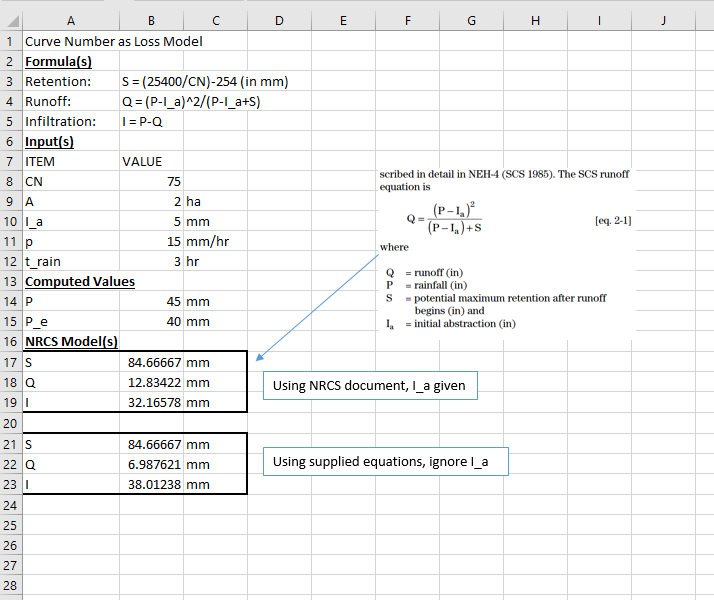
\includegraphics[width=6in]{es3-6xls.png} 
   \caption{Excel screen capture for ES3-6}
   \label{fig:es3-6xls}
\end{figure}
\clearpage
\begin{figure}[h!] %  figure placement: here, top, bottom, or page
   \centering
   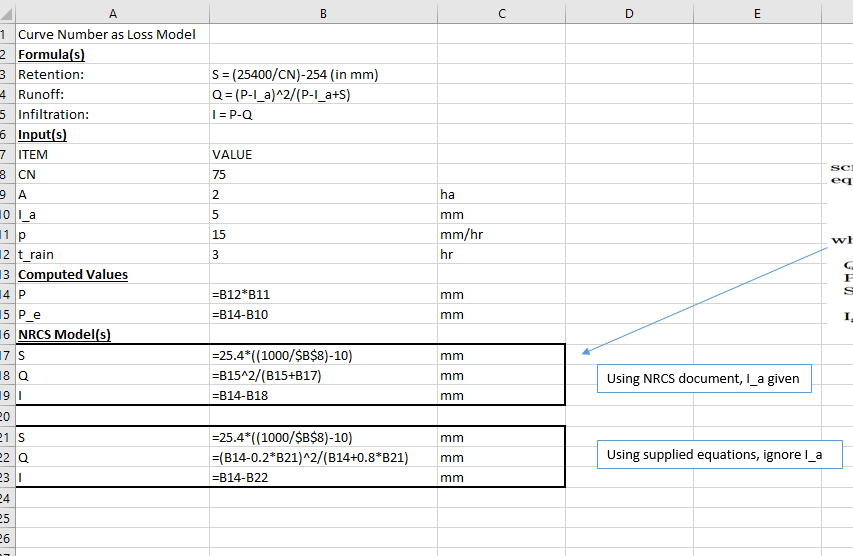
\includegraphics[width=6in]{es3-6func.png} 
   \caption{Excel screen capture for ES3-6 (formulas)}
   \label{fig:es3-6func}
\end{figure}


\clearpage

    \item Compare infiltration results among the three methods.
    \begin{enumerate}[a)]
        \item What causes the differences?

\textsl{The three models are built on different assumptions and emphasize different aspects of infiltration. CN Model is empirical and event-based, lumping all losses into a single abstraction value derived from land use and antecedent conditions. It assumes infiltration is front-loaded and limited by a fixed potential maximum retention.\\ \\Green-Ampt is a physically based model that assumes a sharp wetting front, constant suction at the wetting front, and uniform soil properties. It models infiltration as a function of cumulative depth and soil moisture gradient.\\ \\ Horton’s equation is semi-empirical, based on observed exponential decay of infiltration capacity over time, reflecting crusting or compaction during rainfall events.}
        \item Which method is most sensitive to changes in soil properties?  

        \textsl{Green-Ampt is the most sensitive to soil properties because it explicitly uses Hydraulic conductivity, Suction head at the wetting front, and Moisture deficit (or porosity). Changes in texture, compaction, or porosity directly affect the infiltration curve.\\ \\ In contrast, Horton abstracts these effects into empirical decay constants, and CN wraps them into look-up tables, making them less directly sensitive.}
        \item How would the results change under wet antecedent conditions?

        \textsl{CN Model incorporates this directly through the Antecedent Moisture Condition (AMC), which reduces retention and increases runoff. Green-Ampt responds through a smaller initial moisture deficit, which increases infiltration rate early but levels off quickly. Horton’s model assumes initial infiltration capacity is lower under wet conditions, so it starts lower and decays to the same minimum. \\ \\ In all models, wetter antecedent conditions generally result in: higher runoff, and lower total infiltration, but the mechanism varies by model.}
        
        \item Suggest which model is most appropriate for:
            \begin{itemize}
                \item Urban drainage design \textsl{CN Method; Simple, conservative, integrates land cover; widely accepted in practice}
                \item Physically-based process modeling. \textsl{Green-Ampt; Captures infiltration physics, adaptable for layered soils and time-varying rainfall}
                \item Regional-scale hydrologic planning \textsl{Horton or CN; Both can be calibrated to regional behavior using observed runoff or soil maps; less parameter-intensive}
            \end{itemize}
    \end{enumerate}
    
\end{enumerate}

\end{document}
